% Options for packages loaded elsewhere
\PassOptionsToPackage{unicode}{hyperref}
\PassOptionsToPackage{hyphens}{url}
\PassOptionsToPackage{dvipsnames,svgnames,x11names}{xcolor}
\documentclass[
  british,
  11pt,
  a4paper,
]{article}
\usepackage{xcolor}
\usepackage[margin=25mm]{geometry}
\usepackage{amsmath,amssymb}
\setcounter{secnumdepth}{-\maxdimen} % remove section numbering
\usepackage{iftex}
\ifPDFTeX
  \usepackage[T1]{fontenc}
  \usepackage[utf8]{inputenc}
  \usepackage{textcomp} % provide euro and other symbols
\else % if luatex or xetex
  \usepackage{unicode-math} % this also loads fontspec
  \defaultfontfeatures{Scale=MatchLowercase}
  \defaultfontfeatures[\rmfamily]{Ligatures=TeX,Scale=1}
\fi
\usepackage{lmodern}
\ifPDFTeX\else
  % xetex/luatex font selection
\fi
% Use upquote if available, for straight quotes in verbatim environments
\IfFileExists{upquote.sty}{\usepackage{upquote}}{}
\IfFileExists{microtype.sty}{% use microtype if available
  \usepackage[]{microtype}
  \UseMicrotypeSet[protrusion]{basicmath} % disable protrusion for tt fonts
}{}
\makeatletter
\@ifundefined{KOMAClassName}{% if non-KOMA class
  \IfFileExists{parskip.sty}{%
    \usepackage{parskip}
  }{% else
    \setlength{\parindent}{0pt}
    \setlength{\parskip}{6pt plus 2pt minus 1pt}}
}{% if KOMA class
  \KOMAoptions{parskip=half}}
\makeatother
\usepackage{color}
\usepackage{fancyvrb}
\newcommand{\VerbBar}{|}
\newcommand{\VERB}{\Verb[commandchars=\\\{\}]}
\DefineVerbatimEnvironment{Highlighting}{Verbatim}{commandchars=\\\{\}}
% Add ',fontsize=\small' for more characters per line
\newenvironment{Shaded}{}{}
\newcommand{\AlertTok}[1]{\textcolor[rgb]{1.00,0.00,0.00}{\textbf{#1}}}
\newcommand{\AnnotationTok}[1]{\textcolor[rgb]{0.38,0.63,0.69}{\textbf{\textit{#1}}}}
\newcommand{\AttributeTok}[1]{\textcolor[rgb]{0.49,0.56,0.16}{#1}}
\newcommand{\BaseNTok}[1]{\textcolor[rgb]{0.25,0.63,0.44}{#1}}
\newcommand{\BuiltInTok}[1]{\textcolor[rgb]{0.00,0.50,0.00}{#1}}
\newcommand{\CharTok}[1]{\textcolor[rgb]{0.25,0.44,0.63}{#1}}
\newcommand{\CommentTok}[1]{\textcolor[rgb]{0.38,0.63,0.69}{\textit{#1}}}
\newcommand{\CommentVarTok}[1]{\textcolor[rgb]{0.38,0.63,0.69}{\textbf{\textit{#1}}}}
\newcommand{\ConstantTok}[1]{\textcolor[rgb]{0.53,0.00,0.00}{#1}}
\newcommand{\ControlFlowTok}[1]{\textcolor[rgb]{0.00,0.44,0.13}{\textbf{#1}}}
\newcommand{\DataTypeTok}[1]{\textcolor[rgb]{0.56,0.13,0.00}{#1}}
\newcommand{\DecValTok}[1]{\textcolor[rgb]{0.25,0.63,0.44}{#1}}
\newcommand{\DocumentationTok}[1]{\textcolor[rgb]{0.73,0.13,0.13}{\textit{#1}}}
\newcommand{\ErrorTok}[1]{\textcolor[rgb]{1.00,0.00,0.00}{\textbf{#1}}}
\newcommand{\ExtensionTok}[1]{#1}
\newcommand{\FloatTok}[1]{\textcolor[rgb]{0.25,0.63,0.44}{#1}}
\newcommand{\FunctionTok}[1]{\textcolor[rgb]{0.02,0.16,0.49}{#1}}
\newcommand{\ImportTok}[1]{\textcolor[rgb]{0.00,0.50,0.00}{\textbf{#1}}}
\newcommand{\InformationTok}[1]{\textcolor[rgb]{0.38,0.63,0.69}{\textbf{\textit{#1}}}}
\newcommand{\KeywordTok}[1]{\textcolor[rgb]{0.00,0.44,0.13}{\textbf{#1}}}
\newcommand{\NormalTok}[1]{#1}
\newcommand{\OperatorTok}[1]{\textcolor[rgb]{0.40,0.40,0.40}{#1}}
\newcommand{\OtherTok}[1]{\textcolor[rgb]{0.00,0.44,0.13}{#1}}
\newcommand{\PreprocessorTok}[1]{\textcolor[rgb]{0.74,0.48,0.00}{#1}}
\newcommand{\RegionMarkerTok}[1]{#1}
\newcommand{\SpecialCharTok}[1]{\textcolor[rgb]{0.25,0.44,0.63}{#1}}
\newcommand{\SpecialStringTok}[1]{\textcolor[rgb]{0.73,0.40,0.53}{#1}}
\newcommand{\StringTok}[1]{\textcolor[rgb]{0.25,0.44,0.63}{#1}}
\newcommand{\VariableTok}[1]{\textcolor[rgb]{0.10,0.09,0.49}{#1}}
\newcommand{\VerbatimStringTok}[1]{\textcolor[rgb]{0.25,0.44,0.63}{#1}}
\newcommand{\WarningTok}[1]{\textcolor[rgb]{0.38,0.63,0.69}{\textbf{\textit{#1}}}}
\usepackage{longtable,booktabs,array}
\newcounter{none} % for unnumbered tables
\usepackage{calc} % for calculating minipage widths
% Correct order of tables after \paragraph or \subparagraph
\usepackage{etoolbox}
\makeatletter
\patchcmd\longtable{\par}{\if@noskipsec\mbox{}\fi\par}{}{}
\makeatother
% Allow footnotes in longtable head/foot
\IfFileExists{footnotehyper.sty}{\usepackage{footnotehyper}}{\usepackage{footnote}}
\makesavenoteenv{longtable}
\usepackage{graphicx}
\makeatletter
\newsavebox\pandoc@box
\newcommand*\pandocbounded[1]{% scales image to fit in text height/width
  \sbox\pandoc@box{#1}%
  \Gscale@div\@tempa{\textheight}{\dimexpr\ht\pandoc@box+\dp\pandoc@box\relax}%
  \Gscale@div\@tempb{\linewidth}{\wd\pandoc@box}%
  \ifdim\@tempb\p@<\@tempa\p@\let\@tempa\@tempb\fi% select the smaller of both
  \ifdim\@tempa\p@<\p@\scalebox{\@tempa}{\usebox\pandoc@box}%
  \else\usebox{\pandoc@box}%
  \fi%
}
% Set default figure placement to htbp
\def\fps@figure{htbp}
\makeatother
\ifLuaTeX
\usepackage[bidi=basic,shorthands=off]{babel}
\else
\usepackage[bidi=default,shorthands=off]{babel}
\fi
\ifLuaTeX
  \usepackage{selnolig} % disable illegal ligatures
\fi
\setlength{\emergencystretch}{3em} % prevent overfull lines
\providecommand{\tightlist}{%
  \setlength{\itemsep}{0pt}\setlength{\parskip}{0pt}}
\usepackage{amsmath,amssymb}
\usepackage{microtype}
\usepackage{xurl}
\usepackage{fancyhdr}
\usepackage{needspace}
\usepackage{float}
\pagestyle{fancy}
\fancyhf{}
\fancyhead[L]{\small Cocoercivity and Douglas--Rachford residual rates}
\fancyhead[R]{\small Research note}
\fancyfoot[C]{\thepage}
\setlength{\headheight}{14pt}
\setlength{\emergencystretch}{3em}
\setcounter{tocdepth}{2}
\let\oldsection\section
\renewcommand{\section}{\Needspace{6\baselineskip}\oldsection}
\let\oldsubsection\subsection
\renewcommand{\subsection}{\Needspace{5\baselineskip}\oldsubsection}

\usepackage{bookmark}
\IfFileExists{xurl.sty}{\usepackage{xurl}}{} % add URL line breaks if available
\urlstyle{same}
\hypersetup{
  pdftitle={Cocoercivity does not give a quadratic residual rate for Douglas--Rachford splitting},
  pdfauthor={Anonymous},
  pdflang={en-GB},
  colorlinks=true,
  linkcolor={black},
  filecolor={Maroon},
  citecolor={Blue},
  urlcolor={teal},
  pdfcreator={LaTeX via pandoc}}

\title{Cocoercivity does not give a quadratic residual rate for
Douglas--Rachford splitting}
\usepackage{etoolbox}
\makeatletter
\providecommand{\subtitle}[1]{% add subtitle to \maketitle
  \apptocmd{\@title}{\par {\large #1 \par}}{}{}
}
\makeatother
\subtitle{Exact counterexamples, the sharp worst-case exponent, and
limits of scalar relaxation}
\author{Anonymous}
\date{5 November 2026}

\begin{document}
\maketitle

\textbf{Status.} Unrefereed, AI-assisted research note. Internal
AI-assisted checking is not external peer review or unaffiliated
reproduction. The contribution and literature boundary are stated in
Section 7. The verification record distinguishes exact finite
certificates, written universal arguments and the external theorems they
use.

\textbf{Version:} 0.1.0-candidate.
\href{https://doi.org/10.5281/zenodo.23990902}{Archived evidence and
DOI}.
\href{https://github.com/ipitchford/douglas-rachford-residual-counterexamples}{Source
and verification package}.

\subsection{Abstract}\label{abstract}

Conjecture 3.5 of Abbaszadehpeivasti and Zamani (2025, version 2)
proposes an order \(N^{-2}\) bound for the squared fixed-point residual
of Douglas--Rachford splitting when one operator is a convex
subdifferential and the other is cocoercive. We give two exact
refutations. A scalar quadratic example defeats part of the stated
overrelaxation range at the second iterate. A two-dimensional cocoercive
rotation defeats the claim at unit relaxation, where the substantive
issue is the absence of gradient structure. For every fixed admissible
stepsize and relaxation parameter, the worst-case squared residual over
the stated class has order \(N^{-1}\). For the \(A=0\) subclass,
allowing arbitrary real scalar multipliers and measuring the final
unrelaxed residual, we derive an exact finite-horizon minimax value
including adaptive and random choices. We also describe prescribed
schedules over linear operators and obtain an elementary exact infimum
for that linear class with multipliers restricted to \((0,2)\). These
latter results combine a classical contraction polynomial inequality,
the known sharp firmly nonexpansive residual bound, and a
rotation-product construction already present in recent literature. A
rational hinge example shows that the full mixed class can exceed the
maximum of a scalar proximal example and the pure linear-rotation
envelope. The paper's separate objective-value acceleration conjectures
remain unresolved.

\subsection{1. Problem and contribution}\label{problem-and-contribution}

Douglas--Rachford splitting seeks a solution of \(0\in Ax+Bx\) by
evaluating resolvents of the two operators separately. This can make a
coupled problem easier to handle. A central theoretical question is how
many updates are needed before the iteration changes very little. Here
we test one proposed uniform guarantee for that stopping quantity, not
the practical speed of all splitting solvers.

All spaces in the stated theorems are finite-dimensional real Euclidean
spaces. The dimension may vary in a worst-case supremum; every lower
construction below needs at most two dimensions. Norms are Euclidean,
and matrix norms are their induced operator norms. Write
\(J_C=(I+C)^{-1}\) for the resolvent of a maximally monotone operator
\(C\), and \(R_C=2J_C-I\) for its reflected resolvent.

Given maximally monotone \(A\) and \(B\), Douglas--Rachford splitting
uses

\[
x^k=J_{\gamma B}w^k,\qquad
y^k=J_{\gamma A}(2x^k-w^k),\qquad
w^{k+1}=w^k+\lambda(y^k-x^k).
\tag{1}
\]

Here \(\gamma>0\) and \(0<\lambda<2\). Let \(T_\lambda\) denote its
fixed-point map. The residual at index \(N\) is

\[r_N=\|T_\lambda w^N-w^N\|=\|w^{N+1}-w^N\|.\]

There are \(N-1\) completed updates before evaluating this residual.
Keeping this convention matters when comparing exact constants.

The residual measures an approximate fixed-point condition for the
splitting variable \(w\). It is not an objective gap or the distance of
the primal shadow \(x=J_{\gamma B}w\) to a solution. Converting it into
those quantities requires further assumptions, such as an appropriate
error bound. The initial-distance normalization below is an analytical
scale, not an implementable stopping test, and update counts do not
account for the cost of evaluating resolvents.

An everywhere-defined operator \(B\) is \(\beta\)-cocoercive when

\[
\langle Bx-By,x-y\rangle\geq\beta\|Bx-By\|^2
\quad\text{for every }x,y.
\tag{2}
\]

This property permits a rotational component; it does not require \(B\)
to be a convex gradient. For a closed proper convex function \(g\), its
subdifferential is denoted \(\partial g\).

The target is Conjecture 3.5 in the inspected latest arXiv version of
Abbaszadehpeivasti and Zamani (2025). Its additional hypotheses are
\(A=\partial g\), \(B\) is \(\beta\)-cocoercive, \(0<\gamma<\beta\), and
\(T_\lambda\) has a fixed point \(w^\star\). It asserts

\[
r_N^2\leq
\frac{\lambda^2}{((N-1)\lambda+1)^2}
\|w^1-w^\star\|^2.
\tag{C}
\]

This note establishes that (C) is false and identifies the correct
uniform exponent under these assumptions. It does not determine the
exact worst-case constant for the entire nonlinear mixed class. The
exact minimax result in Section 5 concerns an explicitly restricted
algorithm class, with \(A=0\).

{\def\LTcaptype{none} % do not increment counter
\begin{longtable}[]{@{}
  >{\raggedright\arraybackslash}p{(\linewidth - 4\tabcolsep) * \real{0.3333}}
  >{\raggedright\arraybackslash}p{(\linewidth - 4\tabcolsep) * \real{0.3333}}
  >{\raggedright\arraybackslash}p{(\linewidth - 4\tabcolsep) * \real{0.3333}}@{}}
\toprule\noalign{}
\begin{minipage}[b]{\linewidth}\raggedright
Result
\end{minipage} & \begin{minipage}[b]{\linewidth}\raggedright
Operator and algorithm class
\end{minipage} & \begin{minipage}[b]{\linewidth}\raggedright
Error measure and conclusion
\end{minipage} \\
\midrule\noalign{}
\endhead
\bottomrule\noalign{}
\endlastfoot
Proposition 1 & Scalar convex quadratics; overrelaxation & Exact failure
of (C) at \(N=2\) \\
Proposition 2 & \(A=0\); cocoercive planar rotation; \(\lambda=1\) &
Exact failure of (C); the fixed instance still converges
geometrically \\
Theorem 4 & Full mixed class in (C); fixed admissible parameters &
Squared update residual has uniform worst-case order \(N^{-1}\), hence
residual norm order \(N^{-1/2}\); no sharp full-class constant \\
Theorem 5 & Linear \(B\), \(A=0\); prescribed real scalars & Exact final
unrelaxed-residual envelope after \(m\) updates \\
Theorem 6 & Possibly nonlinear \(B\), \(A=0\); adaptive real scalars &
Exact unrelaxed-residual minimax after \(m\) updates; not generic mixed
DRS tuning \\
Corollary 6.1 & Linear \(B\), \(A=0\); adaptive scalars in \((0,2)\);
\(c>2\) & Exact minimax infimum, not attained in the open interval \\
Section 6 and Appendix A & Mixed splitting with a hinge and rotation &
Exact finite witnesses against an elementary repair considered here \\
\end{longtable}
}

In the scheduling results \(m=N-1\), but the reported error is
\(\|G(w^m)\|\), without multiplying by a reporting relaxation. This
convention prevents a small scalar from making an unchanged state appear
accurate.

\subsection{2. Two exact
counterexamples}\label{two-exact-counterexamples}

\subsubsection{Proposition 1: a scalar overrelaxation
obstruction}\label{proposition-1-a-scalar-overrelaxation-obstruction}

Set \(\beta=1\), \(\gamma=1/2\), \(\lambda=9/5\), \(B=0\) and
\(g(x)=5x^2\). Thus \(A=10I\), and both operators are subdifferentials
of smooth convex functions. The resolvents are \(J_{\gamma B}=I\) and
\(J_{\gamma A}=I/6\). Consequently,

\[T_\lambda=(1-\lambda)I+\frac{\lambda}{6}I=-\frac12I.\]

With \(w^1=1\) and \(w^\star=0\), the second residual is

\[
|T_\lambda w^2-w^2|^2=\frac9{16}
>\frac{81}{196}
=\frac{\lambda^2}{(\lambda+1)^2}.
\tag{3}
\]

The ratio is \(49/36\). Every parameter lies strictly inside the
proposed intervals. Since the zero operator is \(\beta\)-cocoercive for
every positive \(\beta\), no limiting argument is needed. This
refutation concerns the stated relaxation range. It does not explain
what happens at \(\lambda=1\).

\subsubsection{Proposition 2: the unit-relaxation
obstruction}\label{proposition-2-the-unit-relaxation-obstruction}

Let \(\beta=1\), \(\gamma=1/2\), \(\lambda=1\), \(g\equiv0\), and

\[
B=\frac1{50}
\begin{pmatrix}1&-7\\7&1\end{pmatrix},
\qquad w^1=\begin{pmatrix}1\\0\end{pmatrix},
\qquad w^\star=0.
\tag{4}
\]

Then \(A=\partial g=0\). Direct multiplication gives

\[B^\mathsf TB=\frac{B+B^\mathsf T}{2}=\frac1{50}I.\]

Therefore \(\langle Bh,h\rangle=\|Bh\|^2\) for every \(h\): \(B\) is
exactly 1-cocoercive. It is continuous, everywhere defined and monotone,
hence maximally monotone. It is invertible, so the solution and fixed
point are uniquely zero.

Since \(A=0\) and \(\lambda=1\), the iteration reduces to \(T=J_{B/2}\).
Its matrix is

\[
T=\frac2{205}
\begin{pmatrix}101&7\\-7&101\end{pmatrix},
\quad T^\mathsf TT=\frac{40}{41}I,
\quad (I-T)^\mathsf T(I-T)=\frac1{205}I.
\tag{5}
\]

It follows that, for every positive integer \(N\),

\[
r_N^2=\frac1{205}\left(\frac{40}{41}\right)^{N-1}
=\frac1{200}\left(\frac{40}{41}\right)^N.
\tag{6}
\]

At \(N=20\), (C) would give \(r_{20}^2\leq1/400\). Instead,

\[
\left(\frac{40}{41}\right)^{20}
=\left(1-\frac1{41}\right)^{20}
\geq1-\frac{20}{41}=\frac{21}{41}>\frac12.
\]

Thus (6) is strictly larger than \(1/400\). Its numerical value is
approximately \(0.00305135471429\), compared with \(0.0025\), an excess
of about \(22.05\%\). The numerical value is illustrative; the rational
identities and Bernoulli inequality prove the claim. For this fixed
matrix, the first violating index is \(18\), as checked separately by
exact arithmetic.

The matrix is a positive dilation plus a skew-symmetric rotation. It is
not a convex gradient: its Jacobian is not symmetric. Cocoercivity
controls the rotation without eliminating it. This distinguishes
Proposition 2 from the scalar relaxation issue in Proposition 1. It does
not prove that adding a gradient assumption repairs (C) at unit
relaxation; that possible residual bound is not established here.

\textbf{A necessary distinction.} This fixed example converges
geometrically. It is not an example of a single fixed problem whose
asymptotic residual decays exactly as \(N^{-1/2}\). The uniform lower
bound proved next selects an instance for each horizon.

\subsection{3. The correct worst-case
exponent}\label{the-correct-worst-case-exponent}

\subsubsection{Lemma 3: cocoercivity of the resolvent
residual}\label{lemma-3-cocoercivity-of-the-resolvent-residual}

Let \(B\) be \(\beta\)-cocoercive and \(\gamma>0\). Define

\[
J=J_{\gamma B},\qquad G=I-J,\qquad
c=1+\frac{\beta}{\gamma}>1.
\tag{7}
\]

Then \(G\) is \(c\)-cocoercive, and \(R=I-2cG\) is nonexpansive.

\emph{Proof.} For two inputs write \(z=Jv-Jw\) and \(d=Gv-Gw\). The
resolvent identity gives \(d=\gamma(BJv-BJw)\) and \(v-w=z+d\). Hence

\[
\langle d,v-w\rangle
=\langle d,z\rangle+\|d\|^2
\geq\left(\frac\beta\gamma+1\right)\|d\|^2.
\]

Expanding \(\|(v-w)-2cd\|^2\) proves nonexpansiveness. This is the
standard resolvent averagedness relationship; see Giselsson (2017,
Proposition 5.2), after translating the reciprocal cocoercivity
convention. We include the proof to fix the constants. \(\square\)

\subsubsection{\texorpdfstring{Theorem 4: order \(N^{-1}\) is sharp
under the conjecture's
assumptions}{Theorem 4: order N\^{}\{-1\} is sharp under the conjecture's assumptions}}\label{theorem-4-order-n-1-is-sharp-under-the-conjectures-assumptions}

Fix \(\beta>0\), \(0<\gamma<\beta\) and \(0<\lambda<2\), and set
\(c=1+\beta/\gamma\). Let \(W_N\) be the supremum of \(r_N^2\) over the
class in Section 1, with \(\|w^1-w^\star\|\leq1\). For

\[N\geq\frac{c^2}{\lambda(2c-\lambda)},\qquad N\geq2,\]

one has

\[
\frac{\lambda}{2c-\lambda}\frac{(N-1)^{N-1}}{N^N}
\leq W_N\leq\frac{\lambda}{(2-\lambda)N}.
\tag{8}
\]

In particular, \(W_N=\Theta(N^{-1})\) for every fixed admissible triple
of parameters. The proposed order \(N^{-2}\) cannot hold with any
uniform constant on this class.

\emph{Upper bound.} Put \(S=R_{\gamma A}R_{\gamma B}\), a nonexpansive
map. Then \(T_\lambda=(1-\lambda/2)I+(\lambda/2)S\). The averaged-map
identity gives

\[
\|T_\lambda w-w^\star\|^2
\leq\|w-w^\star\|^2
-\frac{2-\lambda}{\lambda}\|T_\lambda w-w\|^2.
\tag{9}
\]

Summing (9) for \(k=1,\ldots,N\) bounds the sum of squared residuals by
\(\lambda/(2-\lambda)\). Nonexpansiveness of \(T_\lambda\) makes the
residual norms nonincreasing. Thus \(Nr_N^2\) is at most this sum. This
is a standard Fejér-monotonicity argument, not a new general upper
bound.

\emph{Lower bound.} Take \(A=0\) and identify the real plane with the
complex numbers. Let \(G\) multiply by a complex number \(z\) satisfying

\[\operatorname{Re}z=c|z|^2,\qquad q=|z|^2\in[0,c^{-2}].\]

Then \(B=\gamma^{-1}G(I-G)^{-1}\) is a real linear \(\beta\)-cocoercive
operator. To check this, \(I-G\) is invertible because \(|z|\leq1/c<1\),
and its multiplier \(b=z/[\gamma(1-z)]\) satisfies

\[
\operatorname{Re}b
=\frac{(c-1)q}{\gamma|1-z|^2}
=\beta|b|^2.
\tag{10}
\]

The relaxed map multiplies by \(1-\lambda z\). Starting at a unit
vector,

\[
r_N^2=\lambda^2q\,[1-\lambda(2c-\lambda)q]^{N-1}.
\tag{11}
\]

Choose \(q=1/[\lambda(2c-\lambda)N]\), which lies in the allowed
interval under the theorem's condition. Substitution proves the lower
bound. Finally,

\[N\frac{(N-1)^{N-1}}{N^N}=\left(1-\frac1N\right)^{N-1}\longrightarrow e^{-1},\]

so both sides of (8) have the claimed order. \(\square\)

The horizon-dependent lower examples can each be strongly monotone and
geometrically convergent, while their strong-monotonicity moduli
deteriorate as the horizon grows. There is no contradiction with
linear-rate theorems that impose a uniform positive modulus.

The exact leading constant for the full mixed class remains unknown
here. In particular, the lower constant in (8) is not asserted to be a
universal sharp constant.

\begin{figure}
\centering
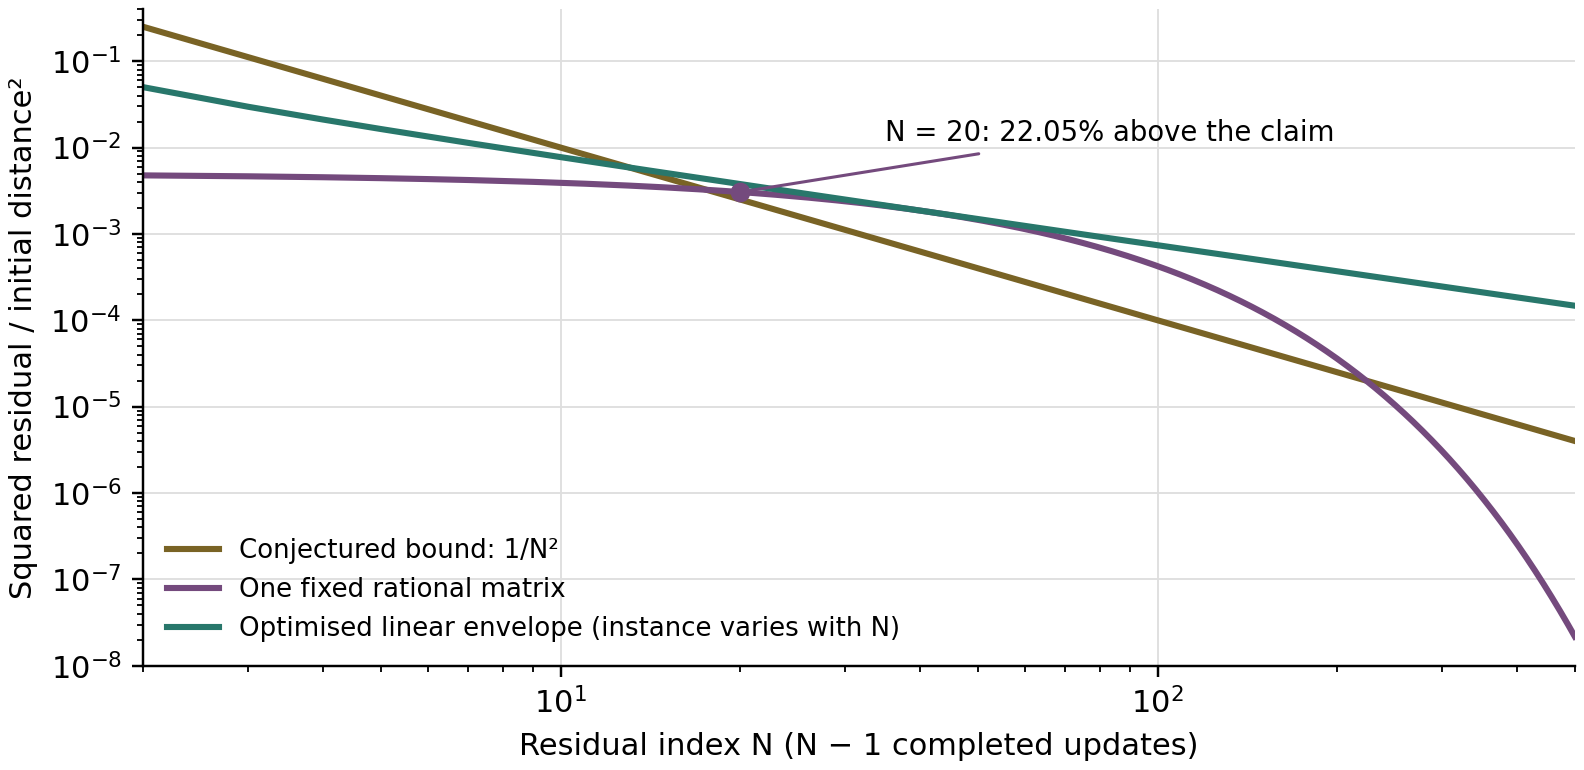
\includegraphics[width=0.95\linewidth,height=\textheight,keepaspectratio,alt={At \textbackslash beta=1, \textbackslash gamma=1/2, \textbackslash lambda=1, the fixed rational witness crosses the proposed bound at finite horizons and eventually decays geometrically. The optimised linear envelope uses a different instance at each horizon and has order N\^{}\{-1\}. The curves illustrate exact formulas; the proofs do not rely on the plot.}]{residual_rates.png}
\caption{At \(\beta=1\), \(\gamma=1/2\), \(\lambda=1\), the fixed
rational witness crosses the proposed bound at finite horizons and
eventually decays geometrically. The optimised linear envelope uses a
different instance at each horizon and has order \(N^{-1}\). The curves
illustrate exact formulas; the proofs do not rely on the plot.}
\end{figure}

\subsection{4. Exact performance of prescribed schedules on linear
operators}\label{exact-performance-of-prescribed-schedules-on-linear-operators}

The preceding construction also gives a complete linear-class
calculation. This section is an explicit corollary of contraction
polynomial theory and known rotation constructions. It is useful for
identifying exactly what scalar scheduling can change.

Fix \(A=0\), \(\beta,\gamma>0\), and use the notation (7). Consider
\(m\) updates

\[w^{j+1}=w^j-\lambda_jG(w^j),\qquad j=0,\ldots,m-1.\]

Here the final error measure is the \textbf{unrelaxed} residual
\(\|G(w^m)\|\). This avoids the artificial possibility of shrinking a
reported update by setting its reporting relaxation to zero.

\subsubsection{Theorem 5: every prescribed real scalar
schedule}\label{theorem-5-every-prescribed-real-scalar-schedule}

For any prescribed real numbers \(\lambda_0,\ldots,\lambda_{m-1}\), the
exact supremum of

\[\frac{\|G(w^m)\|^2}{\|w^0-w^\star\|^2}\]

over all finite-dimensional linear \(\beta\)-cocoercive \(B\) and
initial points with \(w^0\ne w^\star\) is

\[
\max_{0\leq q\leq c^{-2}}
q\prod_{j=0}^{m-1}\bigl[1-(2c\lambda_j-\lambda_j^2)q\bigr].
\tag{12}
\]

Each value in the maximisation is attained by a real two-dimensional
operator of the form (10), with scalar endpoints included.

\emph{Proof.} By Lemma 3, \(R=I-2cG\) is a linear contraction. The
residual after \(m\) steps is the polynomial operator

\[p(G)=G\prod_{j=0}^{m-1}(I-\lambda_jG).\]

Von Neumann's polynomial inequality bounds its norm by the maximum of
\(|p(z)|\) over the disk with centre \(1/(2c)\) and radius \(1/(2c)\).
An inspected modern statement and proof are in Hartz (2025, Proposition
2.3), specialised to scalar coefficients. For real matrices, apply the
inequality to their complexification, which preserves the Euclidean
operator norm. The maximum-modulus principle puts the maximum on the
boundary circle \(\operatorname{Re}z=c|z|^2\). On that circle,

\[|1-\lambda_jz|^2=1-(2c\lambda_j-\lambda_j^2)|z|^2.\]

This proves the upper bound (12). Multiplication by a boundary \(z\) on
the real plane attains the scalar expression, and (10) supplies an
admissible \(B\). \(\square\)

For constant \(0<\lambda<2c\), put \(a=\lambda/(2c)\) and \(N=m+1\).
Multiplying (12) by \(\lambda^2\) gives the exact squared
update-residual envelope

\[
E_N(a)=
\begin{cases}
\displaystyle\frac{a}{1-a}\frac{(N-1)^{N-1}}{N^N},
&N\geq[4a(1-a)]^{-1},\\[6pt]
\displaystyle4a^2|1-2a|^{2N-2},
&N<[4a(1-a)]^{-1}.
\end{cases}
\tag{13}
\]

For \(N=1\), the value is \(4a^2\), with the continuous \(0^0=1\)
convention when needed. Equation (13) follows by maximising the
single-variable function in (11); it is not an upper bound for arbitrary
nonlinear mixed splittings.

At \(\beta=1\), \(\gamma=1/2\), \(\lambda=1\), one has \(a=1/6\) and

\[E_N(1/6)=\frac15\frac{(N-1)^{N-1}}{N^N}\quad(N\geq2).\]

\subsection{5. Exact minimax over adaptive scalar
policies}\label{exact-minimax-over-adaptive-scalar-policies}

The word \emph{policy} below concerns only the scalar multiplying the
current residual. It may use the entire history, complete problem
information or internal randomisation. Random policies are assumed
measurable, so the nonnegative residual has a well-defined, possibly
infinite expectation. The iterate must still obey the displayed update,
and the returned point must be the last iterate. Anchoring, a matrix
update, an additional search direction and an averaged or extrapolated
output are outside this class.

In the original regime \(\gamma<\beta\), the scalar \(c=1+\beta/\gamma\)
exceeds two. The next theorem permits that scalar: it concerns \(A=0\)
and unrestricted real multipliers, not generic mixed DRS with relaxation
in \((0,2)\). Its last-iterate error is the unrelaxed residual.
Corollary 6.1 treats the conventional interval only for linear
operators.

\subsubsection{Theorem 6: a sharp adaptive limit and an exact
penalty}\label{theorem-6-a-sharp-adaptive-limit-and-an-exact-penalty}

Fix an integer \(m\geq1\), \(\beta,\gamma>0\), and \(c\) from (7). Over
all policies of the form

\[w^{j+1}=w^j-\lambda_jG(w^j),\qquad\lambda_j\in\mathbb R,\]

the minimax expected squared final residual over all everywhere-defined
\(\beta\)-cocoercive \(B\) with a zero and initial distance at most one
is exactly

\[
\mathcal M_m=\frac1{c^2}\frac{m^m}{(m+1)^{m+1}}.
\tag{14}
\]

The constant policy \(\lambda_j=c\) guarantees this bound uniformly over
all such operators, including nonlinear operators, and attains the
minimax value. A single two-dimensional instance, chosen for the horizon
but independently of the policy, gives the following pathwise identity
for \(w^0\ne0\):

\[
\frac{\|G(w^m)\|^2}{\|w^0\|^2}
=\mathcal M_m
\prod_{j=0}^{m-1}
\left[1+\frac{(\lambda_j/c-1)^2}{m}\right].
\tag{15}
\]

\emph{Lower bound and penalty.} Choose the complex multiplier

\[z_\star=\frac{1+i\sqrt m}{c(m+1)}.\]

It satisfies \(\operatorname{Re}z_\star=c|z_\star|^2\) and corresponds
to an admissible \(B\) through (10). For every real \(\lambda\),

\[
|1-\lambda z_\star|^2
=\frac{m}{m+1}
\left[1+\frac{(\lambda/c-1)^2}{m}\right].
\]

Multiply this identity along the realised trajectory and use
\(|z_\star|^2=1/[c^2(m+1)]\). This proves (15), even when the scalars
depend on the entire preceding trajectory. Every factor is at least one.
Taking expectations proves the lower bound for random policies as well.

\emph{Upper bound.} Lemma 3 makes \(T=I-cG\) firmly nonexpansive. Every
everywhere-defined firmly nonexpansive map \(T\) is the resolvent of the
maximally monotone relation \(T^{-1}-I\). Thus the sharp proximal-point
bound of Gu and Yang (2019), equation (2.6), Proposition 4.1 and
equation (4.4), applies. Their index \(N\) is our \(m\): the measured
difference is between iterates \(m+1\) and \(m\), after \(m\) completed
updates from the initial point. In our notation the inherited bound is

\[
\|(I-T)T^m w^0\|^2
\leq\frac{m^m}{(m+1)^{m+1}}\|w^0-w^\star\|^2.
\tag{16}
\]

Its use here requires no linearity. Since \(I-T=cG\), (16) proves the
matching upper bound. \(\square\)

Equality in (15) requires \(\lambda_j=c\) at every step on this
adversarial instance. This does not make the constant policy the unique
optimal policy on all other instances. A policy may act differently on
easier instances and retain the same worst-case value.

For the original parameter regime \(\gamma<\beta\), one has \(c>2\). The
attaining policy therefore lies outside the generic Douglas--Rachford
interval \(0<\lambda<2\). It is valid for the \(A=0\) cocoercive
subclass, not as a proposed universal choice for nonzero \(A\). Even
allowing this enlarged scalar-policy class does not improve the order
beyond \(m^{-1}\) for squared residual. This gives a fortiori a lower
barrier for the smaller policy class.

Theorem 6 is a synthesis with an exact refinement. Sarkar and Aggarwal
(2026, Appendix A) already derive the corresponding rotation product for
prescribed Krasnoselskii--Mann schedules; Gu and Yang supply (16). The
exact adaptive quantifiers and the penalty identity were not located
together in the inspected literature. That bounded finding does not
establish historical priority.

\subsubsection{Corollary 6.1: conventional-range scalar policies on the
linear
subclass}\label{corollary-6.1-conventional-range-scalar-policies-on-the-linear-subclass}

Let \(c>2\) and \(m\geq1\). Restrict to finite-dimensional linear
\(\beta\)-cocoercive \(B\), set \(A=0\), and normalize the initial
distance to a zero by one. Allow adaptive or randomized policies as in
Theorem 6, but require every realized scalar to lie in the open interval
\((0,2)\). The infimum, over these policies, of the worst-case expected
squared final \textbf{unrelaxed} residual is

\[
L_m=\max_{0\leq q\leq c^{-2}}q[1-4(c-1)q]^m
=
\begin{cases}
\displaystyle\frac{m^m}{4(c-1)(m+1)^{m+1}},
&m+1\geq\displaystyle\frac{c^2}{4(c-1)},\\[6pt]
\displaystyle c^{-2}\left(\frac{(c-2)^2}{c^2}\right)^m,
&m+1<\displaystyle\frac{c^2}{4(c-1)}.
\end{cases}
\tag{16a}
\]

No admissible policy attains this infimum. Constant scalars tending to
two from below approach it.

\emph{Proof.} Put \(d=4(c-1)\). Since \(c>2\), we have \(dc^{-2}<1\).
Let \(q_*>0\) maximize the displayed continuous function and choose once
a planar boundary multiplier \(z\) with \(\operatorname{Re}z=c|z|^2\)
and \(|z|^2=q_*\). The construction (10) gives an admissible linear
\(B\) with zero at the origin. Choose a unit initial point. For every
realized \(\lambda\in(0,2)\), the function \(2c\lambda-\lambda^2\) is
strictly increasing on this interval and strictly smaller than \(d\).
Hence, pathwise,

\[
\|G(w^m)\|^2
=q_*\prod_{j=0}^{m-1}[1-(2c\lambda_j-\lambda_j^2)q_*]
>q_*(1-dq_*)^m=L_m.
\]

The same instance is used for every policy at this horizon. All factors
on the right are positive, so the strict inequality holds for every
realization, even when the scalars depend on full problem information.
Its expectation is strictly larger than \(L_m\) (or infinite). Thus
every admissible policy has worst-case expected residual strictly larger
than \(L_m\), proving both the lower bound on the infimum and
nonattainment.

Conversely take deterministic constant policies \(\lambda_j=\ell\) with
\(0<\ell<2\). Theorem 5 gives their exact linear-class worst-case value
as \(\max_{0\leq q\leq c^{-2}}q[1-(2c\ell-\ell^2)q]^m\). As
\(\ell\uparrow2\) the functions converge uniformly on this compact
interval to \(q(1-dq)^m\). Their maxima therefore converge to \(L_m\),
proving the matching upper bound on the infimum.

Finally, \(\frac{d}{dq}\{q(1-dq)^m\}=(1-dq)^{m-1}[1-d(m+1)q]\). The
maximizer is \(q_*=1/[d(m+1)]\) if this lies in \([0,c^{-2}]\), and
otherwise is \(q_*=c^{-2}\). Substitution gives (16a); the two formulas
agree at the threshold. \(\square\)

This is an elementary consequence of the existing rotation product and
linear polynomial bound, not a separate major novelty claim. It supplies
a lower barrier for any larger operator class containing these linear
examples. It does \textbf{not} provide a matching upper bound for
nonlinear \(B\) or for nonzero \(A\), and the excluded boundary scalar
\(\lambda=2\) is not an admissible attaining policy.

\subsection{6. A hinge example beyond the two elementary
envelopes}\label{a-hinge-example-beyond-the-two-elementary-envelopes}

The lower family in Theorem 4 does not exhaust the finite-horizon
behaviour of the mixed class. At \(\beta=1\), \(\gamma=1/2\),
\(\lambda=1\), take

\[
B=\frac1{65}\begin{pmatrix}1&-8\\8&1\end{pmatrix},
\quad g(x)=\frac{10}{59}\max\{x_1,0\},
\quad w^1=\begin{pmatrix}1\\2/25\end{pmatrix}.
\tag{17}
\]

Again \(B^\mathsf TB=(B+B^\mathsf T)/2=I/65\), so \(B\) is 1-cocoercive.
The origin is the unique solution because \(B\) is strongly monotone and
\(0\in\partial g(0)\). The proximal map of a scalar hinge
\(h(t)=a\max\{t,0\}\) is exactly

\[
\operatorname{prox}_{\gamma h}(v)=
\begin{cases}
v,&v<0,\\
0,&0\leq v\leq\gamma a,\\
v-\gamma a,&v>\gamma a.
\end{cases}
\tag{18}
\]

Apply (18) to the first coordinate and leave the second coordinate
unchanged. Ten direct rational iterations give

\[
\frac{r_{10}^2}{\|w^1\|^2}
=0.0100992483946696\ldots>\frac1{100}.
\tag{19}
\]

The decimal is only a readable representation. The accompanying
certificate computes the rational numerator and denominator from (1),
tests every branch of (18), and verifies the strict comparison after
cross multiplication. This same example exceeds the pure linear-rotation
envelope \(E_{10}(1/6)\approx0.00774841\). It therefore rules out an
elementary repair considered in this note: taking only the maximum of
\(N^{-2}\) and the rotation envelope. This repair is not attributed to
an external conjecture. No complete mixed-class envelope is claimed.

The construction combines a rotation with a constant hinge subgradient
over part of the trajectory. An exact terminal active-set analysis and
numerical performance-estimation work guided its choice. Neither the
discovery computation nor the exploratory optimisation is needed to
replay the finite certificate.

Appendix A gives an analytic family that already violates the
unit-relaxation bound at \(N=9\), with a fully rational instance at
parameter \(t=1/100\). It explains how a small rotation perturbs a
scalar hinge extremiser. The small exact gap exposes an active-set
mechanism that approximate arithmetic could miss; it is not evidence of
practical instability, divergence or failure of optimisation. No minimal
failure horizon is asserted.

\subsection{7. Literature boundary and remaining
questions}\label{literature-boundary-and-remaining-questions}

\subsubsection{What is established here}\label{what-is-established-here}

Propositions 1 and 2 refute the exact conjecture as printed. Theorem 4
establishes the correct uniform exponent for precisely that operator
class and all fixed admissible parameters. Theorem 5 describes the whole
linear subclass under prescribed scalar schedules. Theorem 6 gives an
exact minimax synthesis for the nonlinear \(A=0\) subclass under
arbitrary real adaptive scalar relaxation. Corollary 6.1 identifies the
linear-subclass infimum for conventional-range adaptive scalars as an
elementary consequence. The hinge certificate excludes a natural but
incomplete finite-horizon repair considered in this note.

\subsubsection{What is inherited from earlier
work}\label{what-is-inherited-from-earlier-work}

The resolvent/cocoercivity correspondence is standard, with directly
relevant formulations in Giselsson (2017). The sharp firmly nonexpansive
residual constant comes from Gu and Yang (2019) and related work of
Lieder. Von Neumann's polynomial inequality is classical. Contreras and
Cominetti (2022) establish an order barrier for prescribed
Krasnoselskii--Mann schedules in general normed spaces. Sarkar and
Aggarwal (2026) explicitly supply the planar rotation product used in a
recent fixed-schedule lower bound. None of these ingredients is
presented as a new discovery.

The mathematical statement of Theorem 6 is more specific than these
inspected statements: its normalisation uses initial distance in
Euclidean space, its constant is exact, and its lower bound holds on one
horizon-dependent instance for every real adaptive policy. Its
derivation is nevertheless short once those earlier ingredients are
combined. This limits the originality claim.

{\def\LTcaptype{none} % do not increment counter
\begin{longtable}[]{@{}
  >{\raggedright\arraybackslash}p{(\linewidth - 2\tabcolsep) * \real{0.5000}}
  >{\raggedright\arraybackslash}p{(\linewidth - 2\tabcolsep) * \real{0.5000}}@{}}
\toprule\noalign{}
\begin{minipage}[b]{\linewidth}\raggedright
Component
\end{minipage} & \begin{minipage}[b]{\linewidth}\raggedright
Contribution and inherited boundary
\end{minipage} \\
\midrule\noalign{}
\endhead
\bottomrule\noalign{}
\endlastfoot
Propositions 1--2 & Explicit refutations of the printed conjecture; the
rotational mechanism itself is established mathematics \\
Theorem 4 & Class-specific sharp exponent from a tailored admissible
lower family and the standard averaged-map upper estimate \\
Theorem 5 & Linear-envelope corollary of the classical contraction
polynomial inequality \\
Theorem 6 & Adaptive-policy formulation and penalty identity synthesized
with an inherited sharp proximal-point upper bound; historical overlap
remains bounded by source access \\
Corollary 6.1 & Elementary restricted-policy linear consequence, not a
new general nonlinear rate \\
Hinge witnesses & Exact finite mixed-class obstruction and analytic
perturbation mechanism; no exact mixed-class envelope or minimal failure
horizon \\
\end{longtable}
}

\subsubsection{Search scope and
missingness}\label{search-scope-and-missingness}

The initial search date was 1 November 2026, with the target version,
proximal-point source, schedule literature and named access gap
rechecked on 5 November 2026. The search covered the originating arXiv
versions and reference list, the publisher and Optimization Online
records, two general web-search systems, exact conjecture-number and
title searches, formula searches for the rotation and residual products,
and the aliases cocoercive equation, averaged operator,
Krasnoselskii--Mann iteration, relaxed proximal point, optimal
relaxation, and step-schedule acceleration. It also checked the current
Evidence Press index for duplicate work. The complete query families,
inspected-source notes and claim decisions accompany this paper.

No prior refutation of Conjecture 3.5 was located. This does not prove
that no such refutation exists. He et al.~(2021), on optimal relaxation
parameters, was available only through its abstract and bibliographic
record. Its exact overlap with the adaptive minimax formulation remains
unverified. Refreshed lawful publisher and repository retrieval attempts
did not obtain the full text. We therefore make no historical-priority
claim for Theorem 6 or its elementary restricted-policy corollary; their
role here is a precisely scoped synthesis accompanying the conjecture
refutation. No author enquiry, subscription-database search or
unaffiliated specialist review occurred. The negative search evidence
supports bounded priority language only.

\subsubsection{Questions left open}\label{questions-left-open}

We do not resolve Conjectures 5.1, 5.6 or 5.7 of the originating paper.
Those concern objective values for convex composite optimisation,
including silver schedules and inertial acceleration. The rotational
counterexample in Proposition 2 does not satisfy their gradient
hypothesis and cannot refute them. The scalar example in Proposition 1
is also not a refutation of those objective bounds.

Additional numerical performance-estimation checks reproduced the
proposed objective bounds at the finite horizons recorded in the
exploratory notes. Such agreement is not a proof. A mirror-coordinate
reformulation exposes the difficulty of a general inertial proof, but
does not close it.

We also leave unresolved the exact mixed-class finite-horizon supremum,
the full nonlinear minimax under the restriction \(0<\lambda_j<2\), and
any fixed-instance asymptotic strengthening. These are different
questions from the proved uniform exponent and the enlarged-policy
minimax theorem.

\subsection{8. Verification and
reproducibility}\label{verification-and-reproducibility}

The main refutations use rational input and can be checked without a
numerical optimiser. The bundle supplies two separately authored exact
implementations, a claim/check ledger, an informal proof outline, a
rating-free assessment and revision response, source notes and a
manifest. The primary certificate uses Python's standard-library
\texttt{fractions.Fraction}; rational equality and inequality checks do
not depend on floating-point tolerances. It reconstructs the updates
from the original resolvent and proximal definitions.

The general theorems are written mathematical arguments. Finite checks
support their algebra and indexing but do not establish their universal
quantifiers. No Lean, Rocq or Isabelle proof was produced. An
independent AI agent re-derived the central rational matrix identities
and the schedule penalty; this is internal cross-checking, not journal
peer review or unaffiliated mathematical validation.

To replay the exact checks from the extracted package, run:

\begin{Shaded}
\begin{Highlighting}[]
\VariableTok{PYTHONDONTWRITEBYTECODE}\OperatorTok{=}\NormalTok{1 }\ExtensionTok{python3} \AttributeTok{{-}B}\NormalTok{ run\_checks.py}
\VariableTok{PYTHONDONTWRITEBYTECODE}\OperatorTok{=}\NormalTok{1 }\ExtensionTok{python3} \AttributeTok{{-}B} \AttributeTok{{-}O}\NormalTok{ run\_checks.py}
\end{Highlighting}
\end{Shaded}

The replay record must identify the exact script versions and whether
normal and optimized execution completed or were rejected. Separately
authored implementations within this project remain producer-side
implementation diversity, not unaffiliated reproduction. The analytic
Appendix A argument, its exact \(t=1/100\) certificate and the optional
symbolic consistency check have different scopes.

A basic sanity check separates the error measures. The conjecture
concerns a \textbf{squared} residual: its proposed \(N^{-2}\)
corresponds to residual norm \(N^{-1}\). Theorem 4's sharp
squared-residual order \(N^{-1}\) corresponds to residual norm
\(N^{-1/2}\). The counterexample does not claim failure of convergence.

\subsubsection{Availability and
declarations}\label{availability-and-declarations}

The accompanying evidence package contains the source manuscript,
exact-check scripts, retained outputs and source-comparison notes. It
uses constructed mathematical examples, not personal or
human-participant data; human-subject ethical approval is not
applicable. Mathematical development, exposition and internal checking
were AI-assisted. The scholarly byline is Anonymous; publication
authority does not imply a human mathematical contribution. No
additional human CRediT role is asserted. No external research grant or
competing interest has been reported in the supplied provenance; these
are reporting limits, not independently verified absence claims.

\subsection{Appendix A. An analytic nine-evaluation hinge
family}\label{appendix-a.-an-analytic-nine-evaluation-hinge-family}

\textbf{Proposition A.1.} At \(\beta=1\), \(\gamma=1/2\) and
\(\lambda=1\), there is a rational-parameter family of two-dimensional
admissible instances for which

\[
\frac{\|T(w_t^9)-w_t^9\|^2}{\|w_t^1\|^2}
=\frac1{81}+\frac5{729}t^2+O(t^4)
\quad\text{as }t\downarrow0.
\tag{A.1}
\]

Consequently the proposed bound fails for every sufficiently small
positive \(t\) in this family.

\emph{Construction.} Write \(e=(1,0)^\mathsf T\) and
\(H=\left(\begin{smallmatrix}0&-1\\1&0\end{smallmatrix}\right)\). Define

\[
B_t=\frac{t^2I+tH}{1+t^2},
\qquad
Q_t=(I+B_t/2)^{-1}
=\frac1{4+9t^2}
\begin{pmatrix}4+6t^2&2t\\-2t&4+6t^2\end{pmatrix},
\]

\[
\begin{aligned}
R_t&=2Q_t-I,& S_t&=\sum_{j=0}^{7}Q_t^j,\\
D_t&=e^\mathsf T R_tS_te+1,& w_t^1&=(1,t/2)^\mathsf T,\\
\delta_t&=\frac{e^\mathsf T R_tQ_t^8w_t^1}{D_t},&
g_t(x)&=2\delta_t\max\{x_1,0\}.
\end{aligned}
\tag{A.2}
\]

Every expression is rational for rational \(t\). Moreover,
\(B_t^\mathsf TB_t=(B_t+B_t^\mathsf T)/2\), so \(B_t\) is 1-cocoercive.
For \(t>0\) it is strongly monotone. Once \(\delta_t>0\), the function
\(g_t\) is convex and the origin is the unique solution and fixed point.

\emph{Proximal branches.} All quantities in (A.2) are analytic near zero
because \(D_0=9\). In particular, \(\delta_0=1/9>0\). Consider the
candidate affine updates

\[w^{k+1}=Q_t w^k-\delta_t e.\]

At \(t=0\), their proximal outputs have first coordinates \(1-k/9\),
which are strictly positive for \(k=1,\ldots,8\). Continuity preserves
those eight active branches for all sufficiently small positive \(t\).
The definition of \(\delta_t\) gives the exact terminal equality

\[
e^\mathsf T\bigl[R_t(Q_t^8w_t^1-\delta_t S_te)-\delta_t e\bigr]=0.
\]

Thus the ninth proximal input has first coordinate \(\delta_t>0\),
exactly the endpoint of the zero branch in (18), and its proximal output
has first coordinate zero. Induction proves that the candidate affine
updates coincide with the actual DRS iteration through the ninth update.

\emph{Residual calculation.} The final residual norm is
\(\|K_t w_t^1\|\), where

\[
K_t=Q_t^8\left[I-Q_t+
\frac{e(e^\mathsf T R_tQ_t^8)}{D_t}\right].
\tag{A.3}
\]

Indeed, \(w_t^9=Q_t^8w_t^1-\delta_t S_te\) and \((I-Q_t)S_t=I-Q_t^8\).
Substituting these identities into \((I-Q_t)w_t^9+\delta_t e\) proves
(A.3).

Expanding the rational matrices gives

\[
Q_t^8=I-4tH-13t^2I+O(t^3),\qquad
S_t=8I-14tH-35t^2I+O(t^3),
\]

\[D_t=9-61t^2+O(t^4),\]

and hence

\[
K_t=
\begin{pmatrix}
1/9+t^2/324&t/18\\
t/18&19t^2/36
\end{pmatrix}
+
\begin{pmatrix}
O(t^4)&O(t^3)\\
O(t^3)&O(t^4)
\end{pmatrix}.
\]

Multiplying by \(w_t^1=(1,t/2)^\mathsf T\), squaring and dividing by
\(1+t^2/4\) gives (A.1). The even remainder follows from the parity of
the rational matrices: diagonal entries are even and off-diagonal
entries are odd in \(t\). Since \(5/729>0\), the strict violation
follows. \(\square\)

The standard-library certificate
\textbf{optimisation\_hinge\_n9\_exact.py} checks \(t=1/100\), including
the eight strict branch inequalities, the ninth exact boundary equality
and the strict comparison to \(1/81\). Its ratio to the conjectured
bound is approximately \(1.00005518699093\). The expansion also has a
separate symbolic consistency check. Neither result establishes a
minimal possible failure horizon or an exact mixed-class envelope.

\subsection{References}\label{references}

\begingroup\small

\subsubsection{Target and operator-splitting
foundations}\label{target-and-operator-splitting-foundations}

Abbaszadehpeivasti, H., \& Zamani, M. (2025). \emph{On the convergence
rate of the Douglas--Rachford splitting algorithm} (Version 2)
{[}Preprint{]}. arXiv. \url{https://arxiv.org/abs/2509.06676v2}

Giselsson, P. (2017). Tight global linear convergence rate bounds for
Douglas--Rachford splitting. \emph{Journal of Fixed Point Theory and
Applications, 19}, 2241--2270.
\url{https://doi.org/10.1007/s11784-017-0417-1}

Gu, G., \& Yang, J. (2019). \emph{Optimal nonergodic sublinear
convergence rate of proximal point algorithm for maximal monotone
inclusion problems} (Version 2) {[}Preprint{]}. arXiv.
\url{https://arxiv.org/abs/1904.05495v2}

Lieder, F. (2021). On the convergence rate of the Halpern-iteration.
\emph{Optimization Letters, 15}, 405--418.
\url{https://doi.org/10.1007/s11590-020-01617-9}

\subsubsection{Scheduling and nearby prior
art}\label{scheduling-and-nearby-prior-art}

Contreras, J. P., \& Cominetti, R. (2022). \emph{Optimal error bounds
for nonexpansive fixed-point iterations in normed spaces} (Version 3)
{[}Author manuscript{]}. \url{https://arxiv.org/abs/2108.10969v3}

He, S., Dong, Q.-L., Tian, H., \& Li, X.-H. (2021). On the optimal
relaxation parameters of Krasnosel'ski--Mann iteration.
\emph{Optimization, 70}(9), 1959--1986.
\url{https://doi.org/10.1080/02331934.2020.1767101} {[}Abstract
inspected; full text unavailable.{]}

Sarkar, D., \& Aggarwal, V. (2026). \emph{Non-expansive two-time-scale
stochastic approximation: A fixed-schedule one-quarter barrier and
bias-corrected acceleration} {[}Preprint{]}. arXiv.
\url{https://arxiv.org/abs/2607.13414}

\subsubsection{Classical polynomial
bound}\label{classical-polynomial-bound}

Hartz, M. (2025). On von Neumann's inequality on the polydisc.
\emph{Mathematische Annalen, 391}, 5235--5264.
\url{https://doi.org/10.1007/s00208-024-03040-2}

von Neumann, J. (1950). Eine Spektraltheorie für allgemeine Operatoren
eines unitären Raumes. \emph{Mathematische Nachrichten, 4}(1--6),
258--281. \url{https://doi.org/10.1002/mana.3210040124} {[}Year follows
the publisher metadata; the work is also conventionally cited as 1951.
The contraction inequality was inspected in Hartz (2025).{]}

\endgroup

\end{document}
